
%!TEX option = --shell-escape

\documentclass[9pt, xcolor={svgnames, x11names},professionalfonts]{beamer}


% \usetikzlibrary{decorations.markings, decorations.fractals}
% \usetikzlibrary{shapes.callouts,shapes.multipart}
% \usetikzlibrary{positioning}

% \setlength{\TPHorizModule}{1.0cm}
% \setlength{\TPVertModule}{\TPHorizModule}

\usepackage{xcolor}
\usepackage{cancel}
\usepackage{bm}
\usepackage{graphicx}
\usepackage{hyperref}
\usepackage{adjustbox}
\hypersetup{colorlinks, allcolors=.,urlcolor=structure}
\usepackage{booktabs}  % for top and bottom spacing in table cells, \addlinespace
\usepackage[x11names, svgnames]{xcolor} % for colors in handouts, auto loaded in Beamer?
\usepackage{tikz}
\usetikzlibrary{arrows.meta, math, calc, shadows,bending}
\usetikzlibrary{decorations.markings, decorations.fractals, decorations.text} % for chain, etc.
\usetikzlibrary{intersections}
\usepackage{pgfmath}
\usepackage{ifthen}
\usepgfmodule{oo}
\usetikzlibrary{shadings}
% \usetikzlibrary{decorations.shapes}
\usepackage[many]{tcolorbox}
\tcbuselibrary{skins} % for image boxes
\usepackage[absolute,overlay,showboxes]{textpos}
% \usepackage{textpos}
% \textblockorigin{0.0cm}{0.0cm}  %start all at upper left corner
\TPshowboxesfalse

\newcommand\lb{\linebreak}
\newcommand\Ra{\Rightarrow}
\newcommand\cd{\!\cdot\!}
\newcommand\x{\!\times\!}
\newcommand\pars{\par\smallskip}
\newcommand\parm{\par\medskip}
\newcommand\parb{\par\bigskip}
\renewcommand{\deg}{^\circ}

% counter for resuming enumerated list numbers
\newcounter{resumeenumi}
\newcommand{\suspend}{\setcounter{resumeenumi}{\theenumi}}
\newcommand{\resume}{\setcounter{enumi}{\theresumeenumi}}



% https://tex.stackexchange.com/questions/33703/extract-x-y-coordinate-of-an-arbitrary-point-in-tikz
\makeatletter
\providecommand{\gettikzxy}[3]{%
	\tikz@scan@one@point\pgfutil@firstofone#1\relax
	\edef#2{\the\pgf@x}%
	\edef#3{\the\pgf@y}%
}
\makeatother

\makeatletter
\newcommand{\verbatimfont}[1]{\def\verbatim@font{#1}}%
\makeatother

%%%%%%%%%%%%%%%%%%%%%%%%%%%%%%%%%%%%%%%%%%%%%%%%%%%%%%%%%%%%%%%%%%%%%%%%%%%%%%%%


% \newcommand{\tb}[4][0.8]{
% 	\begin{textblock*}{#1}(#2, #3)
% 		\raggedright
% 		#4
% 	\end{textblock*}
% }

% \def\tb

\newtcolorbox{statsbox}[2][] { 
  colback=white,
  colbacktitle=structure,
  colframe=structure,
  coltitle=white,  
  top=0.25cm,
	bottom=0.125cm,
	left=0mm,
	right=0mm,
  % fonttitle=\itshape\rmfamily,
  halign=flush left, 
  enhanced,
  drop fuzzy shadow,
  attach boxed title to top left={xshift=3.5mm, yshift=-2mm},
  title={#2}, #1}
\newtcolorbox{redbox}{colback=white, colframe=structure, enhanced, drop fuzzy shadow}
\newtcolorbox{titledbox}[1]{colback=white,colframe=structure,title={#1}}
\newtcbox{\tcb}[1][]{colback=white,boxsep=0pt,top=0.5cm,bottom=0.5cm,left=0.5cm,
		right=0.5cm, colframe=structure,  enhanced, drop fuzzy shadow, #1}
\newtcbox{\tcbfig}[1][1]{colback=white,boxsep=0pt,top=0.5cm,bottom=0.5cm,left=0.5cm,
		right=0.5cm, colframe=structure,  enhanced, drop fuzzy shadow, #1}
% tcb title
\newtcbox{\tcbt}[2][]{colback=white,boxsep=0pt,top=5pt,bottom=5pt,left=5pt,
		right=5pt, colframe=structure, enhanced, drop fuzzy shadow,  title={#2}, #1}
% tcb left title
\newtcbox{\tcbtl}[2][]{ colback=white,
  colbacktitle=structure,
  colframe=structure,
  coltitle=white,  
  top=0.25cm,
	bottom=0.125cm,
	left=0mm,
	right=0mm,
  % fonttitle=\bfseries,
  halign=flush left, 
  enhanced,
  drop fuzzy shadow,
  attach boxed title to top left={xshift=3.5mm, yshift=-2mm}, 
	title={#2}, #1}

\newtcbtheorem{myexam}{Example}%
{
	enhanced,
	colback=white,
	colframe=structure,
	% fonttitle=\bfseries,
	fonttitle=\itshape\rmfamily,
	drop fuzzy shadow,
	%description font=\mdseries\itshape,
	attach boxed title to top left={yshift=-2mm, xshift=5mm},
	colbacktitle=structure
	}{exam}% then \pageref{exer:theoexample} references the theo

% \newcommand{\myexample}[2][red]{
% 	% \tcb\tcbset{theostyle/.style={colframe=red,colbacktitle=yellow}}
% 	\begin{myexam}{}{}
% 		#2
% 	\end{myexam}
% 	% \tcbset{colframe=structure,colbacktitle=structure}
% }

\newtcbtheorem{myexer}{Exercise}%
{
	enhanced,
	colback=white,
	colframe=structure,
	% fonttitle=\bfseries,
	drop fuzzy shadow,
	fonttitle=\itshape\rmfamily,
	% description font=\mdseries\itshape,
	attach boxed title to top left={yshift=-2mm, xshift=5mm},
	colbacktitle=structure
	}{exer}



\newcommand{\mini}[2][0.8]{
	\begin{minipage}[c]{#1\columnwidth}
		\raggedright
		#2
	\end{minipage}
}
\newcommand{\minit}[2][0.8]{
	\begin{minipage}[t]{#1\columnwidth}
		% \raggedright
		#2
	\end{minipage}
}

% centered minipage with text \raggedright
%\cmini[width]{content}
\newcommand{\cmini}[2][0.8]{
	\begin{center}
		\begin{minipage}{#1\columnwidth}
			\raggedright
			#2
		\end{minipage}
	\end{center}
}

\newcommand{\fig}[2][1]{% scaled graphic
	\includegraphics[scale=#1]{#2}
}

% centred framed box black border
%\cbox[width]{content}
\newcommand{\cbox}[2][1]{% framed centered color box
	\setlength\fboxsep{5mm}
	\setlength\fboxrule{.2 mm}
	\begin{center}
		\fcolorbox{black}{white}{
			\vspace{-0.5cm}
			\begin{minipage}{#1\columnwidth}
				\raggedright
				#2
			\end{minipage}
		}
	\end{center}
	\setlength\fboxsep{0cm}
}

\newcommand{\ccbox}[4][1]{% framed centered color box
	\setlength\fboxsep{5mm}
	\setlength\fboxrule{.2 mm}
	\begin{center}
		\fcolorbox{#2}{#3}{
			% \vspace{-0.5cm}
			\begin{minipage}{#1\columnwidth}
				\vspace{-0.25cm}
				\raggedright				
				#4
				\vspace{-0.325cm}
			\end{minipage}
		}
	\end{center}
	\setlength\fboxsep{0cm}
}

\newcommand{\cfig}[2][1]{% centred, scaled graphic
	\begin{center}
		% \fcolorbox{structure}{white}{
		\tcbincludegraphics{
			\includegraphics[scale=#1]{#2}
		}
	\end{center}
}

% figure with tight border for photos
% \cfigb[saitMaroon]{borderwidth with unit}{scale}{image}
\newcommand{\stcsfig}[2][1]{
	% \usepackage{adjustbox}
	% \setlength{\fboxrule}{1pt}
	\begin{center}
		\tcbincludegraphics[width=#1\textwidth, boxrule=2pt, top=-3pt, right=-3pt, left=-3pt, bottom=-3pt,colframe=structure, sharp corners, enhanced, drop fuzzy shadow]{#2}
	\end{center}
}






 \definecolor{saitPurple}{RGB}{112,40,119}
 \definecolor{statsMaroon}{rgb}{0.55, 0, 0}
 \definecolor{saitMaroon}{rgb}{0.55, 0, 0}
 \definecolor{saitRed}{RGB}{224,38,37}
 \definecolor{saitBlue}{rgb}{0, 0.59, 0.85}
 \definecolor{statsDeepBlue}{RGB}{0, 99, 167}
 \definecolor{saitDeepBlue}{RGB}{0, 99, 167}
 \definecolor{LightGrey}{RGB}{200,200,200}
%  \definecolor{boxBG}{RGB}{236, 227, 227}
%  \definecolor{boxBG}{RGB}{242, 233, 223}
% !TEX root = ../Beamer/02ForceVectors/02ForceVectors.tex


\newcommand{\EyeBolt}[6][0]{
	\def\lrotate{#1};
	\def\lpin{#2}
	\def\lfill{#3}
	\def\ldraw{#4}
	\def\lscale{#5}
	\def\lwidth{#6}
	%\def\h{1.5}
	\def\r{0.3}
	\begin{scope}[scale=\lscale, rotate=\lrotate]
		\filldraw[draw=\ldraw, fill=\lfill, line width=\lwidth pt] ($(\lpin) + (-0.7,-1.25)$) arc(180:90:.2) -- ++(0.05,0)arc(-90:0:0.2) -- ++(0.05,0.65)arc(225:-45:0.28284)-- ++(0.05,-.65)arc(180:270:.2)-- ++(0.05,0)arc(90:0:0.2) -- cycle;
		\fill[outer color=\lfill, inner color=black, line width = 0] (\lpin) circle (2.25mm);
		\filldraw[fill=white, draw=\ldraw, line width = \lwidth pt] (\lpin) circle (1.25mm);

		\begin{scope}[even odd rule]
			\fill[\lfill] (\lpin) circle (2.5mm)
			(\lpin) circle (2.125mm);
		\end{scope}

		\filldraw[rounded corners=\lscale pt, draw=\ldraw, fill=\lfill, line width=\lwidth pt] ($ (\lpin) - (1,1.5) $) rectangle +(2,0.25);
	\end{scope}
}

% !TEX root = ../../Beamer/statikz/statikz.tex


\newcommand{\EyeConnection}[6][0]{
	\def\lrotate{#1};
	\def\lpin{#2}
	\def\lfill{#3}
	\def\ldraw{#4}
	\def\lscale{#5}
	\def\lwidth{#6}
	\def\h{1}
	\def\r{0.3}
	\begin{scope}[scale=\lscale, rotate=\lrotate]
		\filldraw[draw=\ldraw, fill=\lfill, line width=\lwidth pt] ($(\lpin) + (0.201*\h+1.0353*\r ,-0.75*\h)$) -- ++(105: 0.77646*\h+0.26795*\r) arc (15:165:\r) -- ++(-105:0.77646*\h+0.26795*\r) -- cycle;

		\fill[outer color=\lfill, middle color=red, inner color=black, line width = \lwidth pt] (\lpin) circle (2.5mm);
		\filldraw[fill=white, draw=\ldraw, line width = \lwidth pt] (\lpin) circle (1.25mm);

		\filldraw[rounded corners=\lscale pt, draw=\ldraw, fill=\lfill, line width=\lwidth pt] ($ (\lpin) - (1,1) $) rectangle +(2,0.25);
	\end{scope}
}

%\Member{startpt}{endpt}{outer fill color}{inner fill color}{stroke}{height}{radius}{linewidth}
\providecommand{\Member}[8]{
  % name the points
  \coordinate(start) at (#1);
  \coordinate(end) at (#2);
  \edef\ofill{#3}%
  \edef\ifill{#4}%
  \edef\stroke{#5}%
  \edef\height{#6} % cm
  \edef\radius{#7} % cm
  \edef\linewidth{#8} % mm

  \coordinate(delta) at ($ (end)-(start) $);
  \gettikzxy{(delta)}{\dx}{\dy}
  \gettikzxy{(start)}{\sx}{\sy}
  \pgfmathparse{veclen(\dx, \dy)} \let\length\pgfmathresult

  \pgfmathparse{\dx==0}%
  % \ifnum low-level TeX for integers
  \ifnum\pgfmathresult=1 % \dx == 0
    \pgfmathsetmacro{\rot}{\dy > 0 ? 90 : -90}
  \else
    \pgfmathsetmacro{\rot}{\dx > 0 ? atan(\dy / \dx) : 180 + atan(\dy / \dx)}
  \fi

  
   
  \shadedraw[transform canvas = { rotate around = {\rot:(\sx,\sy)}}, line width = \linewidth, rounded corners = \radius mm, top color = \ofill, bottom color = \ofill, middle color = \ifill, draw = \stroke] ($ (start)+(-0.5*\height, 0.5*\height) $) -- ++(\height cm +\length pt, 0 ) -- ++(0, -\height) -- ++ (-\height cm -\length pt, 0) -- cycle;


  \shadedraw[ball color = \ofill!50!\ifill, draw = \stroke] (start) circle (\height/8);
  \shadedraw[ball color = \ofill!50!\ifill, draw = \stroke] (end) circle (\height/8);
  %  \pgfresetboundingbox

  
  


}


\newcommand{\PC}[6][0]{%
  \edef\lrotate{#1}%
  \edef\lpin{#2}%
  \edef\lfill{#3}%
  \edef\ldraw{#4}%
  \edef\lscale{#5}%
  \edef\lwidth{#6}%
  \edef\h{1}%
  \edef\r{0.3}%
  \begin{scope}[scale=\lscale, rotate=\lrotate]
	\filldraw[draw=\ldraw, fill=\lfill, line width=\lwidth mm] ($ (\lpin) + (0.201*\h+1.0353*\r ,-0.75*\h) $) -- ++(105: 0.77646*\h+0.26795*\r) arc (15:165:\r) -- ++(-105:0.77646*\h+0.26795*\r) -- cycle;

	\shadedraw[ball color=\lfill, draw=\ldraw, line width = \lwidth mm] (\lpin) circle (1.5mm);

	\filldraw[rounded corners=\lscale pt, draw=\ldraw, fill=\lfill, line width=\lwidth mm] ($ (\lpin) - (1,1) $) rectangle +(2,0.25);
  \end{scope}%
}



% !TEX root = ../Beamer/statikz/statikz.tex

% \Ring{A}{outer color}{inner color}{outer radius}{inner radius}{line width}
\newcommand{\Ring}[6]{
	\def\lpin{#1}
	\def\lfill{#2}
	\def\ldraw{#3}
	\def\outerr{#4}
	\def\innerr{#5}
	\def\lwidth{#6}

	\begin{scope}

		\makeatletter
		\providecommand{\gettikzxy}[3]{%
			\tikz@scan@one@point\pgfutil@firstofone#1\relax
			\edef#2{\the\pgf@x}%
			\edef#3{\the\pgf@y}%
		}
		\makeatother

		\gettikzxy{(\lpin)}{\cx}{\cy}
		\pgfdeclareradialshading{ring}{\pgfpoint{0cm}{0cm}}
		{
			color(0cm)=(black);
			color(0.5cm)=(\lfill);
			color(.65cm)=(\ldraw);
			color(1cm)=(\lfill)
		}
		% \pgfuseshading{ring}



	\end{scope}


\begin{scope}[even odd rule]
	% \draw (\lpin) circle (\innerr);
	\filldraw[shading=ring, fill=\lfill, draw=\ldraw, line width=\lwidth] (\lpin) circle (\outerr cm)
		(\lpin) circle (\innerr);
		\draw[black, line width = \lwidth mm] (\lpin) circle (\innerr cm);
		\draw[black, line width = \lwidth mm] (\lpin) circle (\outerr cm);
\end{scope}


}


\setlength{\parindent}{0pt}
\setlength{\parskip}{\medskipamount}


\tcbset{fonttitle=\itshape\rmfamily}
\usepackage{mathpazo}
 
\usepackage{pgfplots}
\pgfplotsset{compat=1.18}
\usefonttheme[onlymath]{serif} % this needs to be before structureitalicserif?
\usefonttheme{structureitalicserif} %make titles fancy ;-)
% 

\usecolortheme[named=statsMaroon]{structure}
\setbeamertemplate{navigation symbols}{} % remove navigation symbols
\setbeamertemplate{headline}{\vspace{0.125cm}}
\setbeamertemplate{footline}{ \hfill \insertshorttitle\qquad \insertsection \qquad \insertframenumber/\inserttotalframenumber\quad{ }\vspace{0.125cm}}
\setbeamertemplate{items}[default]
\setbeamertemplate{blocks}[shadow=true]

\setbeamercolor{title}{bg=statsMaroon, fg=Azure}
\setbeamercolor{frametitle}{fg=white, bg=statsMaroon}
\setbeamercolor{background canvas}{bg=Gainsboro!50}
\setbeamercolor{block title}{bg=statsMaroon, fg=white}
\setbeamercolor{block body}{bg=white, fg=black}

\setlength{\parskip}{\medskipamount}
\setlength{\parindent}{0pt}

% https://tex.stackexchange.com/questions/731957/how-to-supress-missing-character-there-is-no-u003b-in-font-nullfont
\tracinglostchars=1
\hfuzz 120pt

\def\scale{1}
\newcounter{examnumber}
\newcounter{exernumber}
%test
\resetcounteronoverlays{tcb@cnt@myexam}
\resetcounteronoverlays{tcb@cnt@myexer}
% \newcounter{myexercisecounter}

% Title page details: 
\title[Equilibrium of a Particle/Concurrent Forces]{\Huge 03 Equilibrium of a Particle \\(Concurrent Forces)}
\subtitle[Engineering Statics]{\Large\textcolor{white}{Engineering Statics}}
\author{}
\date{\small Updated on: \today}

% \raggedright

%%%%%%%%%%%%%%%%%%%%%%%%%%%%%%%%%%%%%%%%%%%%%%%%%%%%%%%%%%%%%%%%%%%%%%%%%%%%%%%%

\begin{document}

%%%%%%%%%%%%%%%%%%%%%%%%%%%%%%%%%%%%%%%%%%%%%%%%%%%%%%%%%%%%%%%%%%%%%%%%%%%%%%%%

\begin{frame}[plain]    %don't need footer on titlepage
	\titlepage
\end{frame}

%%%%%%%%%%%%%%%%%%%%%%%%%%%%%%%%%%%%%%%%%%%%%%%%%%%%%%%%%%%%%%%%%%%%%%%%%%%%%%%%

\begin{frame}{Statics and Equilibrium}
	\small
	\begin{itemize}
		\item Mechanics is a branch of physics dealing with bodies that are subject to forces.
		\item Statics is the branch of mechanics that deals with bodies that are in {\bf equilibrium}.
		\item Bodies in equilibrium are either {\bf static} (not moving, or at rest) or are moving with a constant velocity.
		\item In this course, we are interested in the forces necessary to keep a body at rest.
		\item We only consider forces in the plane, i.e. this course is limited to bodies described in only two dimensions (2-D), not those described in space (3-D).
		\item Furthermore, these bodies are assumed to be {\bf rigid}. That is, they do not deform when loads are applied. In practice, structural members {\bf do} deform when loaded but, if correctly designed, deformation is generally minimal and we can ignore the slight geometrical changes.
		\item Unless otherwise noted, structural bodies are presumed to have no weight. We do this because the weight of the body is generally small compared to the loads imposed. %A wooden residential truss can support 15-20 times its own weight.
	\end{itemize}

\end{frame}

%%%%%%%%%%%%%%%%%%%%%%%%%%%%%%%%%%%%%%%%%%%%%%%%%%%%%%%%%%%%%%%%%%%%%%%%%%%%%%%%

\begin{frame}{Conditions for Equilibrium }
	\def\scale{0.85}
	\begin{itemize}
		\item In the previous module, we investigated the resultant force $\bm{R}$ of several forces acting at a single point.\pars
		\item $\bm{R}$  is the net force that results from combining these several component forces $\bm{ F _1}$, $\bm{F_2}$, $\bm{F_3},\ldots$
	\end{itemize}
	% \vspace{-0.25cm}
	\mini[0.65]{
		\begin{itemize}
			\item  The resultants that we found have been non-zero.\pars
			\item From Newton's Laws, we know that a net force acting on a particle will cause this particle to accelerate. So, should ring at $\bm A$ be moving? Or are other forces involved that we haven't considered?\pars
			\item The ring at $\bm A$ resists the effects of the two forces $\bm{F}$ and $\bm{G}$, maintaining the ring in its stationary position.
		\end{itemize}
	}
	\hfill
	\mini[0.3]{
		\tcb{\input{../../pikz/02ForceVectors/fv28Mod3.tex}}
	}
	\begin{itemize}
		\item These resisting forces that maintain equilibrium are called {\bfseries reactions}.

	\end{itemize}

\end{frame}

%%%%%%%%%%%%%%%%%%%%%%%%%%%%%%%%%%%%%%%%%%%%%%%%%%%%%%%%%%%%%%%%%%%%%%%%%%%%%%%%



\begin{frame}{Conditions for Equilibrium }

	\mini[0.55]{
		\begin{itemize}
			\item Reactions are necessary for equilibrium to occur in a structure.\parb
			\item When we walk across a room, our weight bears vertically down onto the floor through one or both of our feet. It is the reaction from the floor that stops us crashing down into the room below. And the one below that.\parb
			\item The study of {\bf statics is the study of equilibrium}, so the reactions that maintain equilibrium are an important part of statics.
		\end{itemize}
	}
	\hfill
	% left-aligned minipage with text raggedright
	%mini[width]{content}
	\mini[0.35]{
		\cfig[0.2]{../../images/unicycle}
		\centering\tiny
		By Frankie Fouganthin (Own work) [CC BY-SA 4.0 (http://creativecommons.org/licenses/by-sa/4.0)], via Wikimedia Commons
		
	}
\end{frame}

%%%%%%%%%%%%%%%%%%%%%%%%%%%%%%%%%%%%%%%%%%%%%%%%%%%%%%%%%%%%%%%%%%%%%%%%%%%%%%%%

\begin{frame}{Equation of Equilibrium for a Particle/Concurrent Forces}

	\cmini[0.8]{
		\begin{itemize}
			\item When in equilibrium, there is no resultant: $\bm{\Sigma \mathrm{ F }_{}=0}$
			\item We frequently solve the two equations $\bm{\Sigma \mathrm{ F }_{x}=0}$ and $\bm{\Sigma \mathrm{ F }_{y}=0}$, setting the sum of the $x$ components and the sum of the $y$ components to 0.
			\item Note that with two equations, {\bf we can only solve for two unknowns} (two forces, if the force lines of action are known, or one force and its direction). If there are three unknowns, we cannot find any of them.
			\item Forces whose lines of action pass through a particle, \lb or point, are known as {\bfseries concurrent forces}.
		\end{itemize}
		\parm
		\begin{tcolorbox}[colback=white,colframe=structure, top=0pt,bottom=0pt,left=0pt,
			right=0pt,center title,title=Equations of Equilibrium for Systems of Concurrent Forces]
			\begin{align*}
				\Sigma F_x & = 0 \\
				\Sigma F_y & = 0 \\
			\end{align*}
		\end{tcolorbox}

	}

\end{frame}

%%%%%%%%%%%%%%%%%%%%%%%%%%%%%%%%%%%%%%%%%%%%%%%%%%%%%%%%%%%%%%%%%%%%%%%%%%%%%%%%


\begin{frame}{Concurrent Forces}

	\begin{textblock*}{1\textwidth}(1cm, 2cm)
		\tikz{
			\node at (0,0){
				\fig[0.25]{../../images/2012-07-30-0560-1200}
			};
		}
	\end{textblock*}


	\begin{textblock*}{1\textwidth}(2.3cm,1.7cm)
		\tikz{
			\uncover<2>{
				\draw[statsMaroon, line width = 1mm, -latex] (0,0) -- (153:3);
				\draw[statsMaroon, line width = 1mm, -latex] (0,0) -- (37:3);
				\draw[statsMaroon, line width = 1mm, -latex] (0,0) -- (-29.5:3);
				\draw[statsMaroon, line width = 1mm, -latex] (0,0) -- (50:3);
				\draw[statsMaroon, line width = 1mm, -latex] (0,0) -- (76:3);
				\draw[statsMaroon, line width = 1mm, -latex] (0,0) -- (-120:3);
				\draw[statsMaroon, line width = 1mm, -latex] (0,0) -- (-135:3);
				\draw[statsMaroon, line width = 1mm, -latex] (0,0) -- (-157:3);
				\filldraw[ball color=statsMaroon] (0,0) circle (2mm);
			}
		}
	\end{textblock*}


\end{frame}



%%%%%%%%%%%%%%%%%%%%%%%%%%%%%%%%%%%%%%%%%%%%%%%%%%%%%%%%%%%%%%%%%%%%%%%%%%%%%%%%

\begin{frame}{Equilibrium of Concurrent Forces}
	\cmini[0.9]{
		\begin{itemize}
			\item If a system is in equilibrium, then each part of that system must be in equilibrium (otherwise that part of the system would move).\parm
			
		\end{itemize}\parm
	}
	\vspace{-1em}
	% left-aligned minipage with text raggedright
	%mini[width]{content}
	\mini[0.45]{
		\def\scale{0.65}
		\tcb{
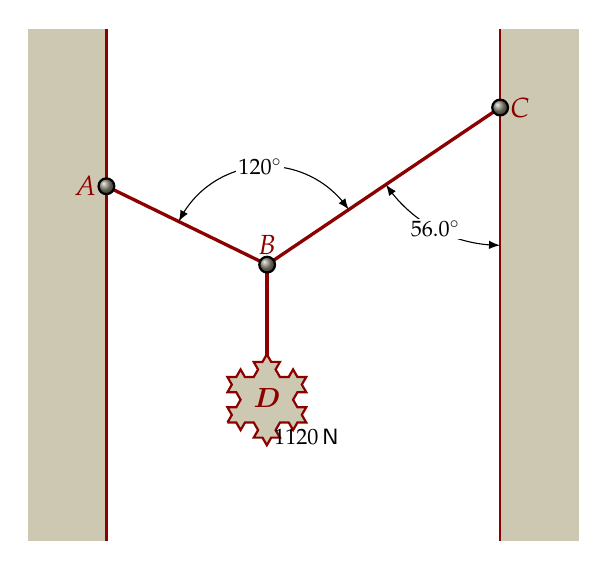
\begin{tikzpicture}[scale=\scale, decoration=Koch snowflake,draw=statsMaroon,fill=Cornsilk3,thick]

	\coordinate (A) at (0,-2);
	\coordinate (AA) at ($(A)+(-26:1)$);
	\coordinate (C) at (5,-1);
	\coordinate (CC) at ($(C)+(214:1)$);
	\coordinate (B) at (intersection of A--AA and C--CC);
	\coordinate (D) at ($ (B)+(0,-1.6875) $);

	\fill[Cornsilk3] ($ (A)+(0,2) $) rectangle  ($ (A)+(-1,-4.5) $); 
	\fill[Cornsilk3] ($ (C)+(0,1) $) rectangle  ($ (C)+(1,-5.5) $); 
	\draw[thick, statsMaroon] ($ (A)+(0,2) $) -- ($ (A)+(0,-4.5) $); 
	\draw[thick, statsMaroon] ($ (C)+(0,1) $) -- ($ (C)+(0,-5.5) $); 


	\draw[very thick, statsMaroon] (A)--(B);
	\draw[very thick, statsMaroon] (B)--(C);
	\draw[very thick, statsMaroon] (B)--(D);

	\filldraw[xshift=1.5375cm, yshift=-2.5cm] decorate{ decorate{ (0,-2.5) -- ++(60:1) -- ++(-60:1) -- cycle }};


	\draw[black, thin, latex-latex] ($ (B)+(154:1.25) $) arc (154:34:1.25) node[fill=white, inner sep=0.25mm, midway] {\footnotesize $120\deg$};
	\draw[black, thin, latex-latex] ($ (C)+(270:1.75) $) arc (270:214:1.75) node[fill=white, inner sep=0.25mm, midway] {\footnotesize $56.0\deg$};


	\shadedraw [draw=black, ball color = Cornsilk4] (B) circle (0.1cm) node[statsMaroon,above] {$B$};
	\shadedraw [draw=black, ball color = Cornsilk4] (A) circle (0.1cm) node[statsMaroon, left] {$A$};
	\shadedraw [draw=black, ball color = Cornsilk4] (C) circle (0.1cm) node[statsMaroon, right] {$C$};
	\node[statsMaroon] at (D) {$\bm D$};
	\node[black, xshift=0.5cm, yshift=-0.5cm] at (D) {\footnotesize $1120\,\mathsf{N}$};



\end{tikzpicture}
}
	}
	\hfill
	\mini[0.5]{
		\begin{itemize}
			\item This system is in equilibrium (it's static).\parm
			\item To solve, break the system down into smaller, separate problems:\parm
			      \begin{enumerate}
			      	\item  Find the force in $BD$\parm
			      	\item Analyze the forces at $B$ to determine the forces in $AB$ and $BC$. (This is the main part of the problem.)\parm
			      	\item Determine the reaction at $A$\parm
			      	\item Determine the reaction at $C$.
			      \end{enumerate}
		\end{itemize}
	}

\end{frame}
%%%%%%%%%%%%%%%%%%%%%%%%%%%%%%%%%%%%%%%%%%%%%%%%%%%%%%%%%%%%%%%%%%%%%%%%%%%%%%%%

%%%%%%%%%%%%%%%%%%%%%%%%%%%%%%%%%%%%%%%%%%%%%%%%%%%%%%%%%%%%%%%%%%%%%%%%%%%%%%%%

\begin{frame}{Actions \& Reactions (Forces Acting on the Pin)}

	%\begin{textblock*}{width, e.g. 3cm}(x-coord eg 1cm, ycoord eg -0.5cm)
	\begin{textblock*}{0.5\textwidth}(6cm, 4.5cm)
		\tikz{
			\node[inner sep=0pt](photo) at (0,0){
				\fig[0.1125]{../../images/2012-07-30-0561-1200}
			};
		}
	\end{textblock*}

	\begin{textblock*}{0.5\textwidth}(0.75cm, 1.5cm)
		\tikz{
			\node[inner sep=0pt](photo) at (0,0){
				\fig[0.35]{../../images/2012-07-30-0565res}
			};
		}
	\end{textblock*}

	\begin{textblock*}{0.5\textwidth}(1.73cm, 2.83cm)
		\tikz{
			\uncover<2->{
				\draw[scale=0.7, line width=1mm, green, -latex] (0,0) -- +(2.5,-1.125);
			}
			\uncover<3->{
				\draw[scale=0.7, line width=1mm, saitRed, -latex] (0,0) -- +(-2.5,1.125);
			}
		}
	\end{textblock*}

	\begin{textblock*}{0.5\textwidth}(9.27cm, 4.45cm)
		\tikz[line cap=round]{
			% \begin{scope}[xshift=4cm, yshift=-1cm]
			%\fill[cyan] (0,0) circle (5pt);
			\uncover<4->{
				\draw[scale=0.7, line width=1mm, green, latex-] (0,0) -- +(0,2);
			}
			\uncover<5->{
				\draw[scale=0.7, line width=1mm, saitRed, latex-] (0,0) -- +(0,-2);
			}
			% \end{scope}
		}
	\end{textblock*}

\end{frame}
%%%%%%%%%%%%%%%%%%%%%%%%%%%%%%%%%%%%%%%%%%%%%%%%%%%%%%%%%%%%%%%%%%%%%%%%%%%%%%%%

\begin{frame}{The Free-Body Diagram}
	\begin{itemize}
		\item An essential part of statics problems is the free-body diagram (\textit{FBD}).
		\item[]\item We need to include all forces acting concurrently (acting on the particle) when using the equations of equilibrium. These forces are shown on the \textit{ FBD}.
		      \parm
		      \begin{enumerate}
		      	\item Isolate the particle from surrounding detail.\parm
		      	\item Draw {\bfseries all} forces that act on the particle: active forces, and the reactive forces that restrict the particle from moving. \parm
		      	\item If the direction of an active or a reactive force is unknown, draw horizontal and vertical components where the reactive force acts. They will be solved later. \parm
		      	\item Forces that are known should be drawn or labelled with their actual magnitude and direction.
		      \end{enumerate}
		\item[]\item Free body diagrams are fairly straightforward for equilibrium of concurrent forces problems.
	\end{itemize}
\end{frame}



%%%%%%%%%%%%%%%%%%%%%%%%%%%%%%%%%%%%%%%%%%%%%%%%%%%%%%%%%%%%%%%%%%%%%%%%%%%%%%%%

\begin{frame}{Solving a Concurrent Force System}

	\begin{myexam}[bottom = 0.375cm]{}{}
		\mini[0.4]{
			\centering
			
			\def\scale{0.65}
			\only<1-9>{
				\vspace{-0.5cm}
				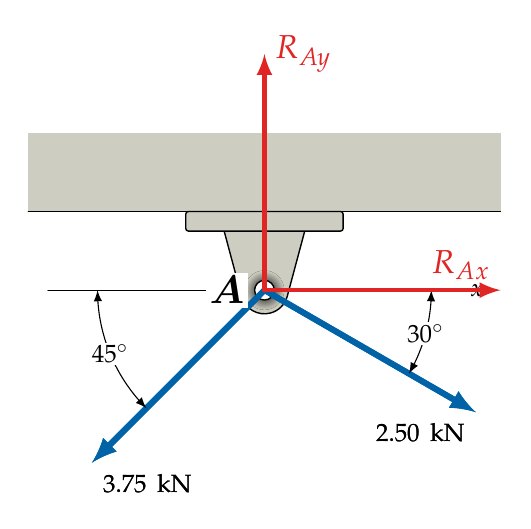
\begin{tikzpicture}[scale=\scale, line cap=round]

	\small

	\coordinate (D) at (-3,1);
	\coordinate (E) at (3, 2);
	\coordinate (C) at (0, 0);	



	\uncover<1-2>{
		\fill[Ivory3] (D) rectangle (E);
		\draw[thin, black] (D) -- ($(E)-(0,1) $);
		\EyeConnection[180]{C}{Ivory3}{black}{1}{0.5};
		\draw[thin] ($(C)+(0.5,0) $) -- +(2,0) node[right] {$x$};
		\draw[line width=0.75mm, -latex, statsDeepBlue] ($ (C)+(-30:.1) $) -- +(-30:3) node[black, below left]{\(2.50\,\text{ kN}\)};
		\draw[line width=0.75mm, -latex, statsDeepBlue] ($ (C)+(225:.1) $) -- +(225:3) node[black, below right]{\(3.75\,\text{ kN}\)};
	}
	\uncover<3-4>{
		\draw[thin] ($(C)+(0.5,0) $) -- +(2.25,0);
	}
	\uncover<3->{
		\draw[thin] ($(C)+(-0.5,0) $) -- +(-2.25,0);
		\draw[line width=0.75mm, -latex, statsDeepBlue] (C) -- +(-30:3.1) node[black, below left]{\(2.50\,\text{ kN}\)};
		\draw[line width=0.75mm, -latex, statsDeepBlue] (C) -- +(225:3.1) node[black, below right]{\(3.75\,\text{ kN}\)};
	}
	
	\uncover<1->{
		\draw[latex-latex] ($ (C)+(180:2.12)$) arc (180:225:2.12) node[fill=white, midway, inner sep=0.25mm] {$ 45\deg $};
		\draw[latex-latex] ($ (C)+(0:2.12)$) arc (0:-30:2.12) node[fill=white, midway, inner sep=0.25mm] {$ 30\deg $};		
	}


	\uncover<5->{
		% \draw[ultra thick, -latex, statsDeepBlue] (C) -- +(-30:3) node[black, below left]{\(2.50\,\text{ kN}\)};
		% \draw[ultra thick, -latex, statsDeepBlue] (C) -- +(225:3) node[black, below right]{\(3.75\,\text{ kN}\)};
		\draw[ultra thick, -latex, saitRed] (C) -- +(0:3) node[above left]{\large $R_{Ax}$};
		\draw[ultra thick, -latex, saitRed] (C) -- +(90:3) node[right]{\large $R_{Ay}$};
	}

	% \only<6->{
	% 	\draw[very thick, -latex, statsMaroon] (C) -- +(0:1) node[right, black]{$0.48659\,$kN};
	% 	\draw[very thick, -latex, statsMaroon] (C) -- +(90:3.5) node[left, black]{$3.9017\,$kN};
	% }
	% \only<7->{
	% 	\draw[gray] ($ (C)+(1,0) $) -- ++(0,3.5) -- +(-1,0);
	% 	\draw[very thick, -latex] (C) -- +(1,3.5) node[right, black]{$R_A$};
	% 	\node at (0.25, 0.25) {$ \theta $};

	% }

		\node at (0,0)[xshift=-0.475cm, fill=white, inner sep=0.5mm] {\Large $\bm A$};





	


\end{tikzpicture}
			}
			\only<10->{
				\begin{tikzpicture}[scale=\scale, line cap=round]

	\small

	\coordinate (D) at (-3,1);
	\coordinate (E) at (3, 2);
	\coordinate (C) at (0, 0);	






	\only<10->{
		\draw[very thick, -latex] (C) -- +(0:1) node[right, black]{$0.48659\,$kN};
		\draw[very thick, -latex] (C) -- +(90:3.5) node[left, black]{$3.9017\,$kN};
	}
	\only<12->{
		
		\draw[gray] ($ (C)+(1,0) $) -- ++(0,3.5) -- +(-1,0);
		\draw[very thick, -latex, saitRed] (C) -- +(1,3.5) node[right]{$R_A$};
		\node at (0.25, 0.25) {$ \theta $};

	}

		\node at (0,0)[xshift=-0.475cm, fill=white, inner sep=0.5mm] {\Large $\bm A$};





	


\end{tikzpicture}
			}
			
		}
		\hfill
		% \vspace{-0.5cm}
		\mini[0.55]{
						
			% \begin{overlayarea}{\columnwidth}{6.75cm}%l}
				\small\vspace{-0.375cm}
				\begin{overlayarea}{\columnwidth}{6.5cm}
				\only<1>{
					\cmini[0.95]{
						\vspace{3cm}
						\begin{flushright}
							Draw an \textit{FBD} for the forces acting at $\bm A$. 
							\pars
							Use this to solve for the reaction at $\bm A$.
						\end{flushright}
						
					}
				}
				\only<2->{
					
					\only<2-6>{
						\vspace{1.125cm}
						Draw the \textit{FBD}:
						\begin{enumerate}				
							\item<2-6> Include {\bf all} the information necessary to solve the problem but omit unnecessary details.
							\item<4-6> It is good practice to draw the reaction components in the direction of the positive axes. Then, if the answer turns out to be negative, you know that the component direction is negative also. 
							\item<6> The \textit{FBD} now has all the information necessary to solve for the reaction.			 	
						\end{enumerate}
					}
					\only<7-9>{
						\parm
						Sum all $x$-components and set to $0$:
						\begin{align*}
							\Sigma F_x &= R_{Ax}+(2.50\,\text{kN})\cd\cos 30\deg \\
							&\qquad\qquad\quad -(3.75\,\text{kN})\cd\cos 45\deg\\
							&= R_{Ax} - 0.48659\,\text{kN} \\
							&=0\quad\text{(for equilibrium)} \\
							\Rightarrow R_{Ax} &= 0.48659\,\text{kN}
						\end{align*}
					}
					\only<8-9>{
						\pars
						Sum all $y$-components and set to $0$:
						\begin{align*}
							\Sigma F_y &= R_{Ay}-(2.50\,\text{kN})\cd\sin 30\deg \\
							&\qquad\qquad\quad -(3.75\,\text{kN})\cd\sin 45\deg\\
							&= R_{Ay} - 3.9017\,\text{kN} \\
							&=0\quad\text{(for equilibrium)} \\
							\Rightarrow R_{Ay} &= 3.9017\,\text{kN}
						\end{align*}
					}
					\only<9>{
						\pars
						Now we can find the reaction from its components.
					}
					\uncover<10->{	
						\par					
						$$ R_{Ax}=0.48659\,\text{kN, }R_{Ay}=3.9017\,\text{kN} $$
					}
					\uncover<11->{%	
					\par\vspace{-0.25cm}						
						Both are positive so the reaction is in the first quadrant. Draw the reaction.
					}
					\uncover<13->{
						% Then:								
						\begin{align*}
							\lvert R_A \rvert &= \sqrt{(R_{Ax})^2+(R_{Ay})^2} \\
							&= \sqrt{\left( 0.48659\,\text{kN} \right)^2+\left( 3.9017\,\text{kN} \right)^2} \\
							&= 3.9319\,\text{kN}
						\end{align*}
					}
					\uncover<14->{
						\vspace{-0.25cm}
						\begin{align*}
							\theta &= \tan^{-1}\left[ \frac{R_{Ay}}{R_{Ax}} \right] \\
							&= \tan^{-1}\left[ \frac{3.9017\,\text{kN}}{0.48659\,\text{kN}} \right]\qquad\quad\;\, \\
							&= 82.891\deg
						\end{align*}
					}						
				}	
				
			\end{overlayarea}					
		}
	\end{myexam}
	\only<15->{
		\begin{textblock*}{\textwidth}(1cm,8.125cm)
			% \TPshowboxestrue
			\centering
			The reaction, $R_A$, at $A$ is $3.93\,\text{kN}$ at $82.9\deg$ (ccw from the positive $x$-axis).
		\end{textblock*}
	}
\end{frame}


%%%%%%%%%%%%%%%%%%%%%%%%%%%%%%%%%%%%%%%%%%%%%%%%%%%%%%%%%%%%%%%%%%%%%%%%%%%%%%%%

\begin{frame}{Solving a Concurrent Force System}



	\begin{myexam}[bottom=0mm, top=2mm]{}{}
		\only<2-3>{
			% \TPshowboxestrue
			\begin{textblock*}{8.75cm}(3cm, 5.92cm)
				\raggedright\footnotesize
				\begin{enumerate}
					\item 	As mentioned before, it is good practice to draw the reaction components in the direction of the positive axes. Then, when our calculations are complete, if the result is positive (if $R_{Ay}>0$), the reaction is in the positive direction. And, then, a negative result (if $R_{Ay}<0$) will always indicate a reaction in the direction of the negative axis.
					\item<3-> $F_{AB}$ drawn pointing away from $A$; the cable is 'pulling' on $A$ and the cable is in tension. Again, it is good practice to always draw unknown forces in tension; then, when the result is positive it follows that the structural member is in tension. A negative result will indicate that member is in compression, 'pushing' on its supports. (Note that cables can only be in tension, never compression. Cables don't push!)
				\end{enumerate}
			\end{textblock*}
		}
		\mini[0.3]{
			\def\scale{0.45}
			
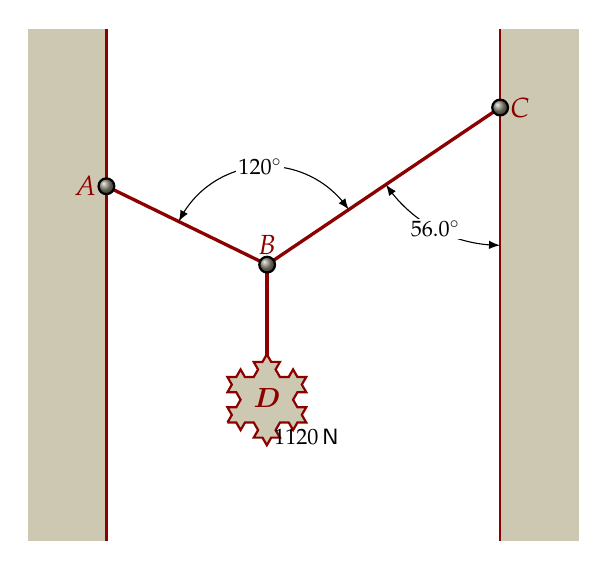
\begin{tikzpicture}[scale=\scale, decoration=Koch snowflake,draw=statsMaroon,fill=Cornsilk3,thick]

	\coordinate (A) at (0,-2);
	\coordinate (AA) at ($(A)+(-26:1)$);
	\coordinate (C) at (5,-1);
	\coordinate (CC) at ($(C)+(214:1)$);
	\coordinate (B) at (intersection of A--AA and C--CC);
	\coordinate (D) at ($ (B)+(0,-1.6875) $);

	\fill[Cornsilk3] ($ (A)+(0,2) $) rectangle  ($ (A)+(-1,-4.5) $); 
	\fill[Cornsilk3] ($ (C)+(0,1) $) rectangle  ($ (C)+(1,-5.5) $); 
	\draw[thick, statsMaroon] ($ (A)+(0,2) $) -- ($ (A)+(0,-4.5) $); 
	\draw[thick, statsMaroon] ($ (C)+(0,1) $) -- ($ (C)+(0,-5.5) $); 


	\draw[very thick, statsMaroon] (A)--(B);
	\draw[very thick, statsMaroon] (B)--(C);
	\draw[very thick, statsMaroon] (B)--(D);

	\filldraw[xshift=1.5375cm, yshift=-2.5cm] decorate{ decorate{ (0,-2.5) -- ++(60:1) -- ++(-60:1) -- cycle }};


	\draw[black, thin, latex-latex] ($ (B)+(154:1.25) $) arc (154:34:1.25) node[fill=white, inner sep=0.25mm, midway] {\footnotesize $120\deg$};
	\draw[black, thin, latex-latex] ($ (C)+(270:1.75) $) arc (270:214:1.75) node[fill=white, inner sep=0.25mm, midway] {\footnotesize $56.0\deg$};


	\shadedraw [draw=black, ball color = Cornsilk4] (B) circle (0.1cm) node[statsMaroon,above] {$B$};
	\shadedraw [draw=black, ball color = Cornsilk4] (A) circle (0.1cm) node[statsMaroon, left] {$A$};
	\shadedraw [draw=black, ball color = Cornsilk4] (C) circle (0.1cm) node[statsMaroon, right] {$C$};
	\node[statsMaroon] at (D) {$\bm D$};
	\node[black, xshift=0.5cm, yshift=-0.5cm] at (D) {\footnotesize $1120\,\mathsf{N}$};



\end{tikzpicture}

		}
		\hfill
		\mini[0.6]{
			\raggedright\footnotesize\vspace{-0.375cm}
			The forces in cables $AB$, $BC$ and $BD$ are concurrent; they act through the single particle/point at $B$.
			\parm
			Draw the \textit{FBD}s for the forces acting upon particles $A$, $B$, $C$ and $D$ in the system shown. \parm
			Then solve for the tensions in the support cables $AB$, $BC$ and $BD$, and the reactions at $A$ and at $C$.
		}
		% don't increment number for next example, it is a continuation of this one
		\addtocounter{\tcbcounter}{-1}
	\end{myexam}
	\parm

	\mini[0.175]{
		\uncover<2->{
			% \centering
			\tcb{				
				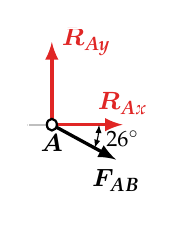
\begin{tikzpicture}[xscale =0.6, yscale=0.7,style={line cap = round}]	
					\small
					\draw [ thick, gray!50] (-.5,0) -- (1.25,0);
					\draw[very thick, black, -latex] (0, 0) -- +(-25:1.5) node [below] { $\bm{F_{AB}}$};
					\draw[very thick, saitRed, -latex] (0, 0) -- +(90:1.5) node [right] { $\bm{R_{Ay}}$};
					\draw[very thick, saitRed, -latex] (0, 0) -- +(0:1.5) node [above] {$\bm{R_{Ax}}$};
					\filldraw[black, fill=white, thick] (0,0) circle (3pt) node [below ] {$\bm{A}$};
					\draw[thin, {Latex[length=3pt]}-{Latex[length=3pt]}] (1, 0) arc [start angle =0, end angle=-25, radius = 1];
					\node at (1.5,-0.25) {\footnotesize $26\deg$};
					\pgfresetboundingbox
					\draw[white] (-0.5,1.75) rectangle (1.875,-1.75);			
				\end{tikzpicture}
			}
		}
	}
	\mini[0.3]{
		\uncover<4->{
			\centering
			\tcb{
				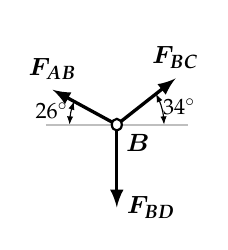
\begin{tikzpicture}[xscale =0.6, yscale=0.7]
					\small				
					\draw [ thick, gray!50] (-1.5,0) -- (1.5,0);
					\draw[very thick,  -latex] (0, 0) -- +(155:1.5) node [above] { $\bm{F_{AB}}$};
					\draw[very thick, -latex] (0, 0) -- +(34:1.5) node [above] { $\bm{F_{BC}}$};
					\draw[very thick, black, -latex] (0, 0) -- (0, -1.5) node [right] { $\bm{F_{BD}}$};
					\filldraw[black, fill=white, thick] (0,0) circle (3pt) node [below right] {$\bm{B}$};
					\draw[thin, {Latex[length=3pt]}-{Latex[length=3pt]}] (1, 0) arc [start angle =0, end angle=34, radius = 1];
					\draw[thin, {Latex[length=3pt]}-{Latex[length=3pt]}] (-1, 0) arc [start angle =180, end angle=155, radius = 1];
					\node at (-1.375,0.26) {\footnotesize $26\deg$};
					\node at (1.325,0.325) {\footnotesize $34\deg$};
					\pgfresetboundingbox
					\draw[white] (-1.875,1.75) rectangle (1.75,-1.75);		
				\end{tikzpicture}
			}
		}
	}
	\mini[0.26]{
		\uncover<5->{
			\tcb{
				
				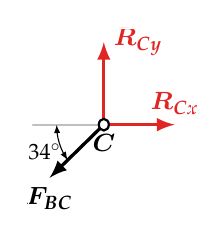
\begin{tikzpicture}[xscale =0.6, yscale=0.7, style={line cap = round}]
					\small					
					\draw [ thick, gray!50] (-1.5,0) -- (1.25,0);
					\draw[very thick, black, -latex] (0, 0) -- +(220:1.5) node [below] { $\bm{F_{BC}}$};
					\draw[very thick, saitRed, -latex] (0, 0) -- +(90:1.5) node [right] { $\bm{R_{Cy}}$};
					\draw[very thick, saitRed, -latex] (0, 0) -- +(0:1.5) node [above] { $\bm{R_{Cx}}$};
					\filldraw[black, fill=white, thick] (0,0) circle (3pt) node [below ] {$\bm{C}$};
					\draw[thin, {Latex[length=3pt]}-{Latex[length=3pt]}] (-1, 0) arc [start angle =180, end angle=220, radius = 1];
					\node at (-1.25,-0.5) {\footnotesize $34\deg$};
					\pgfresetboundingbox
					\draw[white] (-1.6,1.75) rectangle (1.85,-1.75);
				\end{tikzpicture}
			}
		}
	}
	% \begin{textblock*}{7cm}(7cm, 6cm)
	% 	here
	% \end{textblock*}
	\mini[0.15]{
		% \hfill
		\uncover<6->{
			\tcb{
				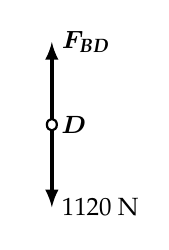
\begin{tikzpicture}[xscale=0.6, yscale=.7]
					\small			
					\draw[very thick,  -latex] (0, 0) -- +(0, 1.5) node [right] { $\bm{F_{BD}}$};
					\draw[very thick, black, -latex] (0,0) -- +(0, -1.5) node [right] { ${\mathrm{ 1120\text{ N} }}$};
					\filldraw[black, fill=white, thick] (0,0) circle (3pt) node [right] {$\bm D$};
					\pgfresetboundingbox
					\draw[white] (-0.5,1.75) rectangle (1.875,-1.75);		
				\end{tikzpicture}
			}
		}
	}
	
\end{frame}
%%%%%%%%%%%%%%%%%%%%%%%%%%%%%%%%%%%%%%%%%%%%%%%%%%%%%%%%%%%%%%%%%%%%%%%%%%%%%%%%

\begin{frame}{Solving for the Tensions and Reactions}
	\cmini[0.825]{
		\begin{myexam}{Analyze $\bm D$}{}
			\raggedright\small
			Each of the \textit{FBD}s for particles $A$, $B$ and $C$ has three unknowns so we cannot solve them yet. We start with $D$.\parb
			\mini[0.3]{
				\centering
				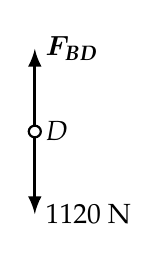
\begin{tikzpicture}[xscale =0.725, yscale=.7]				
					\draw[very thick, -latex] (0, 0) -- +(0, 1.5) node [right] { $\bm{F_{BD}}$};
					\draw[very thick, black, -latex] (0,0) -- +(0, -1.5) node [right] { ${\mathrm{ 1120\text{ N} }}$};
					\filldraw[black, fill=white, thick] (0,0) circle (3pt) node [right] {$D$};
				\end{tikzpicture}
			}
			\hfill
			\mini[0.575]{
				\uncover<2>{
					\small
					\begin{align*}
						\Sigma F_x         & = 0                       \\
						\Sigma F_y         & = F_{BD}-1120\text\,{N}=0 \\
						\Rightarrow F_{BD} & = 1120\,\text{N}
					\end{align*}
				}
			}
			\addtocounter{\tcbcounter}{-1}
		\end{myexam}
	}
\end{frame}

%%%%%%%%%%%%%%%%%%%%%%%%%%%%%%%%%%%%%%%%%%%%%%%%%%%%%%%%%%%%%%%%%%%%%%%%%%%%%%%%

\begin{frame}%{Solving for forces at $D$, $B$, $A$ and $C$}

	\begin{myexam}{Analyze $\bm B$}{}
		\small
		\mini[0.3]{
			
			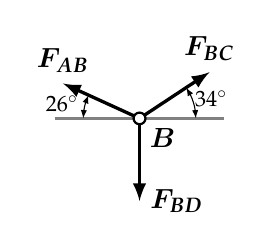
\begin{tikzpicture}[xscale =0.715, yscale=0.7]
				
				\draw [ thick, gray] (-1.5,0) -- (1.5,0);
				\draw[very thick,  -latex] (0, 0) -- +(155:1.5) node [above] { $\bm{F_{AB}}$};
				\draw[very thick,  -latex] (0, 0) -- +(34:1.5) node [above] { $\bm{F_{BC}}$};
				\draw[very thick, black, -latex] (0, 0) -- (0, -1.5) node [right] { $\bm{F_{BD}}$};
				\filldraw[black, fill=white, thick] (0,0) circle (3pt) node [below right] {$\bm{B}$};
				\draw[thin, {Latex[length=3pt]}-{Latex[length=3pt]}] (1, 0) arc [start angle =0, end angle=34, radius = 1];
				\draw[thin, {Latex[length=3pt]}-{Latex[length=3pt]}] (-1, 0) arc [start angle =180, end angle=155, radius = 1];
				\node at (-1.375,0.26) {\footnotesize $26\deg$};
				\node at (1.275,0.35) {\footnotesize $34\deg$};
			\end{tikzpicture}
		}
		\hfill
		\mini[0.6]{			
			Now that we have found that $F_{BD}=1120\,\text{N}$, there are only two unknowns at $B$ and we can proceed. This analysis of particle $B$ involves the solving of two simultaneous equations.
			% \vspace{-0.0625cm}
			\footnotesize
			\begin{align*}				
				\Sigma F_x         & = F_{BC}\cdot\cos 34\deg-F_{AB}\cdot\cos 26\deg = 0 \\
				\Rightarrow F_{BC} & = F_{AB}\cdot\frac{\cos 26\deg}{\cos 34\deg}
			\end{align*}
		}
		% \vspace{-0.25cm}
		\cmini[0.8]{
			\footnotesize
			\begin{align*}
				\uncover<2->{
					\Sigma F_y = F_{AB}\cdot\sin 26\deg + F_{BC}\cdot\sin 34\deg - 1120\text{ N} &= 0    \\
					\Rightarrow F_{AB}\cdot\sin 26\deg + \left[F_{AB}\cdot\frac{\cos 26\deg}{\cos 34\deg}\right]\cdot\sin 34\deg &= 1120\text{ N} \\
					\Rightarrow F_{AB}\left[ \sin 26\deg + \cos 26\deg\tan 34\deg  \right] &= 1120\text{ N} \\
					\Rightarrow F_{AB} &= 1072.2\text{N} \\\\
				}
				\uncover<3->{
					\Rightarrow F_{BC} &= F_{AB}\cdot\frac{\cos 26\deg}{\cos 34\deg}\\
					&= 1072.2\text{N}\cdot\frac{\cos 26\deg}{\cos 34\deg} \\
					&= 1162.4\,\text{N}
				}
			\end{align*}
		}
		\addtocounter{\tcbcounter}{-1}
	\end{myexam}
	\visible<4>{
		\begin{tikzpicture}[remember picture, overlay]
			\fill[white,opacity=0.8] (current page.south west) rectangle (current page.north east);
		\end{tikzpicture}
	}
	\only<4>{
		% \TPshowboxestrue
		\begin{textblock*}{8cm}(4.5cm, 4.5cm)
			\begin{statsbox}{Or use the system-solver?}{}
				\raggedright\footnotesize
				I recommend that you learn how to use the system-solver on your calculator to save time and reduce the chance of errors\ldots
				\parm
				The two equations you enter are: 
				\begin{align*}
					-\cos 26\deg\cdot x +\cos 34\deg\cdot y &= 0 \\
					\sin 26\deg\cdot x + \sin 34\deg\cdot y &= 1120\text{ N} 
				\end{align*}
				where $x$ represents $F_{AB}$ and $y$ represents $F_{BC}$; $x$ and are just algebraic variables used by the calculator and are not related to the $x$ or $y$-axes. These equations are identical to the ones used for the simultaneous equation solution, with $F_{AB}$ and $F_{BC}$ relabeled $x$ and $y$, and a little reordering of terms. 
			\end{statsbox}
		\end{textblock*}
	}
\end{frame}
%%%%%%%%%%%%%%%%%%%%%%%%%%%%%%%%%%%%%%%%%%%%%%%%%%%%%%%%%%%%%%%%%%%%%%%%%%%%%%%%

\begin{frame}%{Solving for forces at $D$, $B$, $A$ and $C$}

	\begin{myexam}{Analyze $\bm A$}{}
		\small
		\mini[0.3]{
			\centering
			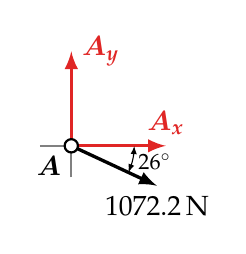
\begin{tikzpicture}[scale=0.8]
				
				\draw [ thick, gray] (-.5,0) -- (0,0);
				\draw [ thick, gray] (0,-0.5) -- (0,0);
				\draw[very thick, black, -latex] (0, 0) -- +(-25:1.5) node [below] { ${1072.2\,}$N};
				\draw[very thick, saitRed, -latex] (0, 0) -- +(90:1.5) node [right] { $\bm{A_{y}}$};
				\draw[very thick, saitRed, -latex] (0, 0) -- +(0:1.5) node [above] { $\bm{A_{x}}$};
				\filldraw[black, fill=white, thick] (0,0) circle (3pt) node [below left] {$\bm{A}$};
				\draw[thin, {Latex[length=3pt]}-{Latex[length=3pt]}] (1, 0) arc [start angle =0, end angle=-25, radius = 1];
				\node at (1.325,-0.25) {\footnotesize $26\deg$};
			\end{tikzpicture}
		}
		\hfill
		\mini[0.65]{
			\footnotesize
			\begin{align*}
				\Sigma F_y      & = A_y-F_{AB}\sin 26\deg = 0     \\
				\Rightarrow A_y & = F_{AB}\sin 26\deg             \\
				                & = (1072.2\,\text{N})\sin 26\deg  \\
				                & = 470.02\,\text{N}                 \\[0.5em]
				\uncover<2->{
					\Sigma F_x      & = A_x + F_{AB}\cos 26\deg = 0   \\
					\Rightarrow A_x & = -(1072.2\,\text{N})\cos 26\deg \\
				                & = -963.69\text\,\text{N}  \\  
				}
			\end{align*}
		}
		\uncover<3->{
			Now, find the resultant, $R_A$, of the two reaction components $A_x$ and $A_y$:\pars
			\mini[0.45]{
				\centering
				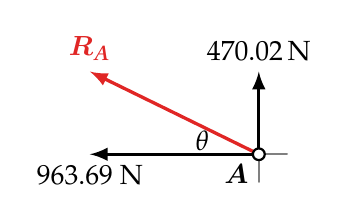
\begin{tikzpicture}[xscale =0.715, yscale=0.7,style={line cap = round}]					
					\draw [ thick, gray] (.5,0) -- (0,0);
					\draw [ thick, gray] (0,-0.5) -- (0,0);
					\draw[very thick, saitRed, -latex] (0, 0) -- +(-3,1.5) node [above] { $\bm{R_{A}}$};
					\draw[very thick, black, -latex] (0, 0) -- +(90:1.5) node [above] { $470.02\,\text{N}$};
					\draw[very thick, black, -latex] (0, 0) -- +(180:3) node [below] {$963.69\text{ N}$};
					\filldraw[black, fill=white, thick] (0,0) circle (3pt) node [below left] {$\bm{A}$};
					\node at (-1,0.25) {$\theta$};
				\end{tikzpicture}
			}
			\hfill
			\mini[0.5]{
				\footnotesize
				\begin{align*}
					R_A    & = \sqrt{(470.02\,\text{N})^2+(963.69\,\text{N})^2}         \\
					       & = 1072.2\text{ N}                                        \\
					\theta & = \tan^{-1}\left(\frac{470.02}{963.69}\right) = 26.000\deg
				\end{align*}
			}
		}
		\uncover<4->{
			\parb\centering
			$R_A$ is equal and opposite to $F_{AB}$, which shouldn't be a surprise.
		}
		\addtocounter{\tcbcounter}{-1}
	\end{myexam}

\end{frame}

%%%%%%%%%%%%%%%%%%%%%%%%%%%%%%%%%%%%%%%%%%%%%%%%%%%%%%%%%%%%%%%%%%%%%%%%%%%%%%%%

\begin{frame}%{Solving for forces at $D$, $B$, $A$ and $C$}

	\begin{myexam}{Analyze $\bm C$}{}
		\mini[0.4]{
			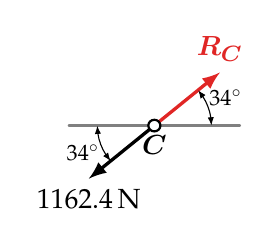
\begin{tikzpicture}[xscale =0.725, yscale=0.7, style={line cap = round}]
				
				\draw [ thick, gray] (-1.5,0) -- (1.5,0);
				\draw[very thick, black, -latex] (0, 0) -- +(220:1.5) node [below] { $1162.4\,\text{N}$};
				\draw[very thick, saitRed, -latex] (0, 0) -- +(40:1.5) node [above] { $\bm {R_C}$};

				% \draw[very thick, saitRed, -latexh] (0, 0) -- +(90:1.5) node [right] { $\bm{C_{y}}$};
				% \draw[very thick, saitRed, -latexh] (0, 0) -- +(0:1.5) node [above] { $\bm{C_{x}}$};
				\filldraw[black, fill=white, thick] (0,0) circle (3pt) node [below ] {$\bm{C}$};
				\draw[thin, {Latex[length=3pt]}-{Latex[length=3pt]}] (-1, 0) arc [start angle =180, end angle=220, radius = 1];
				\node at (-1.25,-0.5) {\footnotesize $34^\circ$};
				\draw[thin, {Latex[length=3pt]}-{Latex[length=3pt]}] (1, 0) arc [start angle =0, end angle=40, radius = 1];
				\node at (1.25,0.5) {\footnotesize $34^\circ$};
			\end{tikzpicture}
		}
		\hfill
		\mini[.5]{
			\small
			Based on our result for the reaction at $A$, it follows that $R_C$ is equal and opposite to $F_{BC}$.\parm
			$R_C$ is $1024\,$N at $34^\circ$, measured counter-clockwise from the positive $x$-axis.
		}	
		\addtocounter{\tcbcounter}{-1}	
	\end{myexam}
	\parm
	\uncover<2->{
		\begin{myexam}{The Answers}{}
			\small
			All rounded to three significant digits:
			$$F_{AB}=1070\,\text{N},\;F_{BC}=1160\,\text{N},\;F_{BD}=1120\,\text{N}$$ 
			$$R_A=1070\,\text{N} \text{ at } 154\deg \text{ ccw from the positive } x\text{-axis}$$
			$$R_C=1160\,\text{N} \text{ at } 34\deg \text{ ccw from the positive } x\text{-axis}$$
			Notice that tension (and compression) do not have a direction. Is the tension in $AB$ from $A$ to $B$ or from $B$ to $A$? Tension and compression are scalar values.
		\end{myexam}
	}
\end{frame}

%%%%%%%%%%%%%%%%%%%%%%%%%%%%%%%%%%%%%%%%%%%%%%%%%%%%%%%%%%%%%%%%%%%%%%%%%%%%%%%%

%%%%%%%%%%%%%%%%%%%%%%%%%%%%%%%%%%%%%%%%%%%%%%%%%%%%%%%%%%%%%%%%%%%%%%%%%%%%%%%%
\begin{frame}{Force Transmissability}

	\begin{itemize}
		\item The {\bf line of action} of a force is the line along the force direction, extended infinitely in both directions.
		\item The effect of a force on a body is the same wherever the force is applied along its line of action.
	\end{itemize}

	\hfill
	\mini[0.31]{
		\centering
		\begin{statsbox}{}
			\centering
			% !TEX root = ../../statikz/statikz.tex


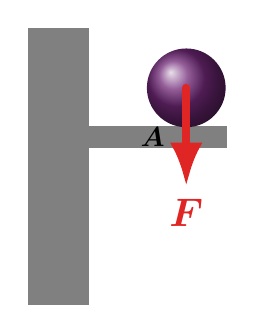
\begin{tikzpicture}
  
  \filldraw [ thick, gray] (0.25,0.25) rectangle (1,3.75);
  \filldraw [ thick, gray] (1,2.25) rectangle (2.75,2.5);
  \shade [ball color = saitPurple] (2.25, 3) circle (0.5cm);
  \draw[line width=1mm, -Latex, saitRed, line cap = round] (2.25, 3) -- (2.25, 1.75) node[below]{\Large$\bm F  $};
  \node at (2.1, 2.375) [left] {$\bm A$};
\end{tikzpicture}

		\end{statsbox}		
	}
	\mini[0.31]{
		\centering
		\begin{statsbox}{}
			\centering
			% !TEX root = ../../statikz/statikz.tex


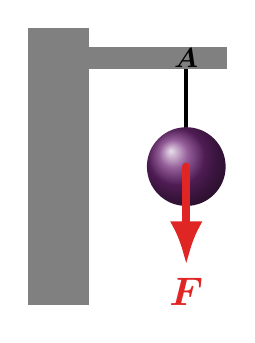
\begin{tikzpicture}

  
  \filldraw [ thick, gray] (0.25,0.25) rectangle (1,3.75);
  \draw [ultra thick] (2.25, 3.25) -- (2.25, 2.25);
  \filldraw [ thick, gray] (1,3.25) rectangle (2.75,3.5);
  \shade [ball color = saitPurple] (2.25, 2) circle (0.5cm);
  \draw[line width=1mm, -Latex, saitRed, line cap = round] (2.25, 2) -- (2.25, 0.75) node[below]{\Large$\bm F $};
  \node at (2.25, 3.375)  {$\bm A$};
\end{tikzpicture}

		\end{statsbox}
	}
	\mini[0.3]{
		\centering
		\begin{statsbox}{}
			\centering
			% !TEX root = ../../statikz/statikz.tex


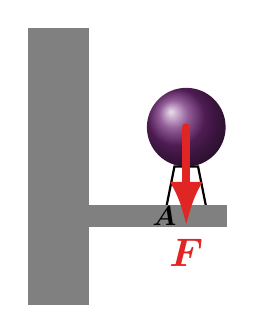
\begin{tikzpicture}
  
  \filldraw [ thick, gray] (0.25,0.25) rectangle (1,3.75);
  \draw [ thick] (2, 1.5) -- (2.1, 2) -- (2.4, 2) -- (2.5, 1.5);
  \filldraw [ thick, gray] (1,1.25) rectangle (2.75,1.5);
  \shade [ball color = saitPurple] (2.25, 2.5) circle (0.5cm);
  \draw[line width=1mm, -Latex, saitRed, line cap = round] (2.25, 2.5) -- (2.25, 1.25) node[below]{\Large$\bm F $};
  \node at (2.25, 1.375) [left] {$\bm A$};
\end{tikzpicture}

		\end{statsbox}
	}

	\begin{itemize}
		\item All these loadings have the same effect on the beam at $A$.
	\end{itemize}
\end{frame}

%%%%%%%%%%%%%%%%%%%%%%%%%%%%%%%%%%%%%%%%%%%%%%%%%%%%%%%%%%%%%%%%%%%%%%%%%%%%%%%%

\begin{frame}{Force Transmissability and Concurrency}

	\begin{textblock*}{1.0\textwidth}(1cm, 3.25cm)
		\begin{tcolorbox}[colframe=structure, colback=white, left=0pt]
			\centering
			\def\scale{0.5}
			
\tikz[line cap=round, scale=\scale]{
	\coordinate (O) at (0,0);
	\coordinate (B) at (-3,3.5);
	\coordinate (C) at (12,0);

	% rectangle
	\filldraw[fill=LightSteelBlue3, draw=black] ($(O)+(-2,2)$) rectangle ($(O)+(5,-2)$);
	\filldraw[fill=white, draw=black] ($(O)+(-1,1)$) rectangle ($(O)+(4,-1)$);
	\fill[inner color=LightSteelBlue4!0.5!black, outer color=LightSteelBlue3, draw=LightSteelBlue3] ($(O)+(-1.5,1.5)$) circle (0.425cm);
	\filldraw[fill=white, draw=black] ($(O)+(-1.5,1.5)$) circle (0.25cm);
	\filldraw[inner color=LightSteelBlue4!0.5!black, outer color=LightSteelBlue3, draw=LightSteelBlue3] ($(O)+(4,1.5)$) circle (0.425cm);
	\filldraw[fill=white, draw=black] ($(O)+(4,1.5)$) circle (0.25cm);
	\fill[inner color=LightSteelBlue4!0.5!black, outer color=LightSteelBlue3, draw=LightSteelBlue3] ($(O)+(0,-1.5)$) circle (0.425cm);
	\filldraw[fill=white, draw=black] ($(O)+(0,-1.5)$) circle (0.25cm);

	\uncover<2->{
		\draw[thick, black] ($(O)+(315:0.5)$)-- +(135:6.5);
		\draw[thick, black] ($(C)+(315:0.5)$)-- +(135:5);
		\draw[thick, black] ($(O)+(90:0.5)$)-- +(270:5.9);
		\draw[thick, black] ($(C)+(90:0.5)$)-- +(270:5);
		\draw[thick, black] ($(O)+(200.56:0.5)$)-- +(20.56:8.64);
		\draw[thick, black] ($(C)+(200.56:0.5)$)-- +(20.56:5);
	}

	\draw[line width=1mm, saitMaroon, -latex] ($(O)+(135:2.1913)$) -- +(135:3);
	\draw[line width=1mm, saitMaroon, -latex] ($(O)+(270:1.57)$) -- +(270:3);
	\draw[line width=1mm, saitMaroon, -latex] ($(O)+(20.56:4.342)$) -- +(20.56:3);

	% ring
	\Ring{C}{LightSteelBlue4}{LightSteelBlue3}{1.75}{0.875}{0.01}
	\draw[line width=1mm, saitMaroon, -latex] ($(C)+(135:0.7)$) -- +(135:3);
	\draw[line width=1mm, saitMaroon, -latex] ($(C)+(270:0.7)$) -- +(270:3);
	\draw[line width=1mm, saitMaroon, -latex] ($(C)+(20.56:0.7)$) -- +(20.56:3);

}
		\end{tcolorbox}
	\end{textblock*}

	\begin{textblock*}{1.0\textwidth}(1.0cm, 1cm)
		\begin{itemize}
			\item If the lines of action of forces go through a single point (or particle), then the forces are concurrent.
			\item Each of the force systems shown is a concurrent system.
			\uncover<2->{Their force lines of action intersect at a single point.}
		\end{itemize}
	\end{textblock*}


\end{frame}

%%%%%%%%%%%%%%%%%%%%%%%%%%%%%%%%%%%%%%%%%%%%%%%%%%%%%%%%%%%%%%%%%%%%%%%%%%%%%%%%

\begin{frame}

	\begin{myexer}{}{}

		\mini[0.45]{
			Determine the reaction at $A$.
		}
		\mini[0.5]{
			% \cfig[0.3]{../../Figs/02ConcurrentForces/conc2016B.png}
		}
		\parm
		\begin{center}
			\footnotesize
			\rotatebox[origin=c]{180}{
				\textcolor{gray}{
					($R=14.9$ kN at $2.91^\circ$ cw from positive $x$ axis.)
				}
			}
		\end{center}
	\end{myexer}

\end{frame}

%%%%%%%%%%%%%%%%%%%%%%%%%%%%%%%%%%%%%%%%%%%%%%%%%%%%%%%%%%%%%%%%%%%%%%%%%%%%%%%%



%%%%%%%%%%%%%%%%%%%%%%%%%%%%%%%%%%%%%%%%%%%%%%%%%%%%%%%%%%%%%%%%%%%%%%%%%%%%%%%%
%%%%%%%%%%%%%%%%%%%%%%%%%%%%%%%%%%%%%%%%%%%%%%%%%%%%%%%%%%%%%%%%%%%%%%%%%%%%%%%%

%%%%%%%%%%%%%%%%%%%%%%%%%%%%%%%%%%%%%%%%%%%%%%%%%%%%%%%%%%%%%%%%%%%%%%%%%%%%%%%%
%%%%%%%%%%%%%%%%%%%%%%%%%%%%%%%%%%%%%%%%%%%%%%%%%%%%%%%%%%%%%%%%%%%%%%%%%%%%%%%%
%%%%%%%%%%%%%%%%%%%%%%%%%%%%%%%%%%%%%%%%%%%%%%%%%%%%%%%%%%%%%%%%%%%%%%%%%%%%%%%%
%%%%%%%%%%%%%%%%%%%%%%%%%%%%%%%%%%%%%%%%%%%%%%%%%%%%%%%%%%%%%%%%%%%%%%%%%%%%%%%%
%%%%%%%%%%%%%%%%%%%%%%%%%%%%%%%%%%%%%%%%%%%%%%%%%%%%%%%%%%%%%%%%%%%%%%%%%%%%%%%%

\end{document}

%%%%%%%%%%%%%%%%%%%%%%%%%%%%%%%%%%%%%%%%%%%%%%%%%%%%%%%%%%%%%%%%%%%%%%%%%%%%%%%%